% Created 2019-08-17 sam. 15:03
% Intended LaTeX compiler: pdflatex
\documentclass[9pt, technote, a4paper]{ieeeconf}
\usepackage[utf8]{inputenc}
\usepackage[T1]{fontenc}
\usepackage{graphicx}
\usepackage{grffile}
\usepackage{longtable}
\usepackage{wrapfig}
\usepackage{rotating}
\usepackage[normalem]{ulem}
\usepackage{amsmath}
\usepackage{textcomp}
\usepackage{amssymb}
\usepackage{capt-of}
\usepackage{hyperref}
\usepackage[most]{tcolorbox}
\usepackage{siunitx}
\usepackage{amsmath,amssymb,amsfonts, cases}
\usepackage{algorithmic, graphicx, textcomp}
\usepackage{xcolor, import, hyperref}
\usepackage[USenglish, english]{babel}
\setcounter{footnote}{1}
\usepackage[utf8]{inputenc}
\usepackage[T1]{fontenc}

\usepackage[french, english]{babel} % Last language is main language

\usepackage{lmodern} % Latin Modern Font
\usepackage{gensymb} % Generic symbols for both text and math mode

\usepackage{standalone} % Used to generate standalone Tikz

\usepackage{amsmath}   % Main math Package
\usepackage{mathtools} % Extension package to amsmath
\usepackage{amsthm}    % Typesetting theorems (AMS style)
\usepackage{amsfonts}  % More fonts from the AMS
\usepackage{textcomp}  % provide many text symbols
\usepackage{steinmetz} % For phase symbol

\usepackage{xstring}  % Utils to manipulate strings
\usepackage{etoolbox} % Add basic if/then
\usepackage{esvect}   % Beautyfull vectors
\usepackage{graphicx} % Enhanced support for graphics
\usepackage{grffile}  % Used by matlab2tikz

\usepackage{microtype} % typographic tuning
\usepackage{setspace}  % for line spacing, e.g. \onehalfspacing
\usepackage{tabularx}  % table features
\usepackage{enumitem}  % for simple list modifications
\usepackage{booktabs}  % better table support

\usepackage{stackengine} %

\usepackage[load-configurations=abbreviations]{siunitx} % SI units
\sisetup{
    locale = US,
    detect-all,
    range-phrase=--,
    range-units=single
}

\usepackage{tikz}       % Tikz
\usepackage{tikzscale}  % Used to scale Tikz graphics
\usepackage{adjustbox}  % Used to proper positioning of tikz pictures
\usepackage{circuitikz} % Draw electronic circuits
\usepackage{pgfpages}   % Needed to use notes
\usepackage{pgfplots}   % Used to plot functions

\usetikzlibrary{arrows}                   % Arrow tip library
\usetikzlibrary{arrows.meta}              % Add some arrows
\usetikzlibrary{calc}                     % The library allows advanced Coordinate Calculations
\usetikzlibrary{intersections}            % calculate intersections of paths
\usetikzlibrary{matrix}                   %
\usetikzlibrary{patterns}                 %
\usetikzlibrary{shapes}                   % Defines circle and rectangle
\usetikzlibrary{shapes.geometric}         % Use for the shape diamond and isosceles triangle
\usetikzlibrary{snakes}                   % snake=coil and snake=zigzag using segment amplitude=10pt
\usetikzlibrary{positioning}              % Additional options for placing nodes
\usetikzlibrary{3d}                       % Plot 3D shapes
\usetikzlibrary{spy}                      % Creating a magnified area
\usetikzlibrary{decorations.text}         % Used to make text follows a curve
\usetikzlibrary{decorations.pathmorphing} % deformation of a path
\usetikzlibrary{decorations.markings}     % Used for spring and damper
\usetikzlibrary{babel}                    % A tiny library that make the interaction with the babel package easier
\usetikzlibrary{plotmarks}                % This library defines a number of plot marks
\usetikzlibrary{fit}                      % Used to make rectangle as nodes by specifying two points
\usetikzlibrary{backgrounds}              % Used to put things under others

\usepgfplotslibrary{patchplots}
\usepgfplotslibrary{groupplots}

\pgfplotsset{compat=newest}
\pgfplotsset{plot coordinates/math parser=false}

\newlength{\fheight}
\newlength{\fwidth}

\setlength{\fwidth}{85mm}
\setlength{\fheight}{112mm}

\tikzset{>=Stealth}
% Setup default Linewidth
\tikzset{every path/.style={line width=1pt}}

\usepackage{xcolor}% Color extension

\definecolor{mycolor1}{RGB}{79,115,193}
\definecolor{mycolor2}{RGB}{213,91,53}
\definecolor{mycolor3}{RGB}{152,126,49}

\tikzset{%
  block/.style n args={2}{%
    draw,
    fill=white,
    minimum width  = #1,
    minimum height = #2,
  },
  block/.default={1.2cm}{1.0cm}
}

\tikzstyle{branch}=[fill,shape=circle,minimum size=4pt,inner sep=0pt]
\tikzstyle{->top}=[-{Stealth[color=black, scale=0.8]}, draw=white, double=black, double distance=1pt, line width=1pt]
\tikzstyle{<-top}=[{stealth[color=black, scale=0.8]}-, draw=white, double=black, double distance=1pt, line width=1pt]

\tikzstyle{handwriten}=[decorate,decoration={random steps,amplitude=0.1pt,segment length=0.8pt}]

\tikzset{%
  DAC/.style={%
    draw,
    signal,
  }
}

\tikzset{%
  ADC/.style={%
    draw,
    signal,
    signal to = west,
  }
}

\tikzset{%
  gain right/.style={%
    draw,
    regular polygon,
    regular polygon sides = 3,
    inner sep = 2pt,
    shape border rotate=-90
  },
  gain left/.style={%
    draw,
    regular polygon,
    regular polygon sides = 3,
    inner sep = 2pt,
    shape border rotate=90
  },
  gain top/.style={%
    draw,
    regular polygon,
    regular polygon sides = 3,
    inner sep = 2pt,
    shape border rotate=0
  },
  gain bottom/.style={%
    draw,
    regular polygon,
    regular polygon sides = 3,
    inner sep = 2pt,
    shape border rotate=180
  },
}

\tikzset{% Add block with Circled operations
  addc/.style n args={5}{%
    draw,
    fill=white,
    circle,
    outer sep = 0pt,
    inner sep = 0pt,
    minimum size = 2em,
    execute at begin node={\LARGE $#1$},
    append after command={\pgfextra{\let\mainnode=\tikzlastnode}
      \ifx#2\empty\else
      node[draw, circle, outer sep=6pt, inner sep=0pt, above left] at (\mainnode.west) {$#2$}%
      \fi
      \ifx#3\empty\else
      node[draw, circle, outer sep=6pt, inner sep=0pt, above right] at (\mainnode.north) {$#3$}%
      \fi
      \ifx#4\empty\else
      node[draw, circle, outer sep=6pt, inner sep=0pt, below right] at (\mainnode.east) {$#4$}%
      \fi
      \ifx#5\empty\else
      node[draw, circle, outer sep=6pt, inner sep=0pt, below left] at (\mainnode.south) {$#5$}%
      \fi
      }
  },
  addc/.default={+}{}{}{}{},
}

\tikzset{% Add Block
  addb/.style n args={5}{%
    draw,
    fill=white,
    circle,
    outer sep = 0pt,
    inner sep = 0pt,
    minimum size = 2em,
    execute at begin node={\LARGE $#1$},
    append after command={\pgfextra{\let\mainnode=\tikzlastnode}
      \ifx#2\empty\else
      node[outer sep=2pt, inner sep=0pt, above left] at (\mainnode.west) {$#2$}%
      \fi
      \ifx#3\empty\else
      node[outer sep=2pt, inner sep=0pt, above right] at (\mainnode.north) {$#3$}%
      \fi
      \ifx#4\empty\else
      node[outer sep=2pt, inner sep=0pt, below right] at (\mainnode.east) {$#4$}%
      \fi
      \ifx#5\empty\else
      node[outer sep=2pt, inner sep=0pt, below left] at (\mainnode.south) {$#5$}%
      \fi
      }
  },
  addb/.default={+}{}{}{}{},
}

\pgfplotsset{
  every axis plot/.append style={line join=round},
  every axis plot/.append style={line cap=round},
}

\pgfplotsset{grid style={black}}
\pgfplotsset{major grid style={black!30!white}}
\pgfplotsset{minor grid style={black!10!white}}
\pgfplotsset{xmajorgrids}
\pgfplotsset{ymajorgrids}

\pgfplotsset{separate axis lines=false} % draw axis as rectangle and not as 4 lines
\pgfplotsset{every outer x axis line/.append style={black}}
\pgfplotsset{every outer y axis line/.append style={black}}
\pgfplotsset{axis background/.style={fill=white}}
\pgfplotsset{axis x line*=bottom} % solid line on the bottom with thin on the top
\pgfplotsset{axis y line*=left} % solid line on the left with thin on the right

\pgfplotsset{every y tick label/.append style={font=\color{black}}}
\pgfplotsset{every y tick/.append style={black}}
\pgfplotsset{every x tick label/.append style={font=\color{black}}}
\pgfplotsset{every x tick/.append style={black}}

\pgfplotsset{scale only axis=true}

\pgfplotsset{ylabel absolute}

% https://tex.stackexchange.com/questions/54794/using-a-pgfplots-style-legend-in-a-plain-old-tikzpicture#54834

% argument #1: any options
\newenvironment{customlegend}[1][]{%
  \begingroup
  % inits/clears the lists (which might be populated from previous
  % axes):
  \csname pgfplots@init@cleared@structures\endcsname
  \pgfplotsset{#1}%
}{%
  % draws the legend:
  \csname pgfplots@createlegend\endcsname
  \endgroup
}%

% makes \addlegendimage available (typically only available within an
% axis environment):
\def\addlegendimage{\csname pgfplots@addlegendimage\endcsname}

% definition to insert numbers
% \pgfkeys{/pgfplots/number in legend/.style={%
%     /pgfplots/legend image code/.code={%
%       \node at (0.125,-0.0225){#1}; % <= changed x value
%     },%
%   },
% }
\pgfplotsset{
  every legend to name picture/.style={west}
}

\tikzset{%
  spring/.style={%
    thick,
    decoration={
      zigzag,
      pre length  = #1cm,
      post length = #1cm,
      segment length = 6
    },
    decorate
  },
  spring/.default={0.2}
}

\tikzset{%
  coil/.style n args={2}{%
    thick,
    decoration={
      coil,
      pre length  = #1cm,
      post length = #2cm,
      segment length = 4
    },
    decorate
  },
  coil/.default={0.3}{0.3}
}

\tikzset{%
  damper/.style n args={2}{%
    thick,
    decoration={markings, mark connection node=dmp, mark=at position 0.5 with {
        \node (dmp) [thick,
                     inner sep = 0pt,
                     transform shape,
                     rotate  =-90,
                     minimum width  = #1pt,
                     minimum height = #2pt,
                     draw=none] {};
        \draw [thick] ($(dmp.north east)+(0.6*#2pt,0)$) -- (dmp.south east) -- (dmp.south west) -- ($(dmp.north west)+(0.6*#2pt,0)$);
        \draw [thick] ($(dmp.north)+(0,-0.3*#1pt)$) -- ($(dmp.north)+(0,0.3*#1pt)$);
      }
    },
    decorate
  },
  damper/.default={12}{3}
}

\tikzset{%
  actuator/.style n args={2}{%
    thick,
    draw=none,
    decoration={
      markings,
      mark connection node=my node,
      mark=at position .5 with {
        \node [draw, inner sep=0pt, minimum width=#1cm, minimum height=#2cm,
        transform shape, fill=white] (my node) {};
      },
      mark=at position .0 with {
        \draw[<-] (0, 0) -- (my node);
      },
      mark=at position 1.0 with {
        \draw[<-] (0, 0) -- (my node);
      }
    },
    decorate
  },
  actuator/.default={0.5}{0.2}
}

\tikzset{%
  ground/.style n args={2}{%
    fill,
    pattern = north east lines,
    draw = none,
    anchor = north,
    minimum width  = #1cm,
    minimum height = #2cm,
    append after command={
      (\tikzlastnode.north west) edge (\tikzlastnode.north east)
    }
  },
  ground/.default={2.5}{0.3}
}

\tikzset{%
  forcesensor/.style n args={2}{%
    rectangle,
    outer sep=0pt,
    inner sep=0pt,
    draw=black,
    fill=white!60!black,
    anchor=south,
    minimum width =#1cm,
    minimum height=#2cm,
    append after command={
      [every edge/.append style={
        thick,
        black,
      }]
      (\tikzlastnode.north west) edge (\tikzlastnode.south east)
      (\tikzlastnode.north east) edge (\tikzlastnode.south west)
    }
  },
  forcesensor/.default={2.0}{0.5}
}

\tikzset{%
  inertialsensor/.style={%
    rectangle,
    outer sep=0pt,
    inner sep=0pt,
    draw=black,
    fill=white!60!black,
    anchor=south east,
    minimum size=#1cm,
    append after command={
      [every edge/.append style={
        thick,
        black,
      }]
      (\tikzlastnode.north west) edge (\tikzlastnode.south east)
      (\tikzlastnode.north east) edge (\tikzlastnode.south west)
    }
  },
  inertialsensor/.default={0.3}
}

\tikzstyle{cross}=[path picture={
  \draw[black]
  (path picture bounding box.south east) -- (path picture bounding box.north west) (path picture bounding box.south west) -- (path picture bounding box.north east);
}]

\tikzset{%
  piezo/.style n args={3}{%
    draw,
    rectangle,
    minimum width  = #1cm,
    minimum height = #2cm,
    fill=blue!10!white,
    anchor=center,
    append after command={
      [every edge/.append style={
        thick,
        black,
      }]
      \foreach \i in {1,...,#3}{
        (${\i/(1+#3)}*(\tikzlastnode.north west)+{(1+#3-\i)/(1+#3)}*(\tikzlastnode.south west)+0.1*(#1,0)$) edge (${\i/(1+#3)}*(\tikzlastnode.north east)+{(1+#3-\i)/(1+#3)}*(\tikzlastnode.south east)-0.1*(#1,0)$)
      }
    }
  },
  piezo/.default={2}{4}{10}
}

\def\voicecoil#1#2#3{
  % ======================
  % Parameters
  % ======================
  \def\voicecoilw{#1} % Total Width
  \def\voicecoilh{#2} % Total Height

  \def\magnetw{\voicecoilw} % Width of the magnet
  \def\magneth{\voicecoilh/1.4} % Height of the magnet

  \def\magnetwb{0.15*\magnetw} % Width of the borders of the magnet
  \def\magnetmw{0.15*\magnetw} % Width of the middle part of the magnet
  \def\magnetwg{0.5*\magnetw} % Width of the gap of the magnet

  \def\magnethl{\magnetwb} % Height of the low part of the magnet
  \def\magnetmh{0.15*\magneth} % Height of the middle part of the magnet
  \def\magnethg{0.2*\magneth} % Height of the gap of the magnet
  % ======================

  \begin{scope}[shift={(0.5*\voicecoilw, 0.5*\voicecoilh)}, rotate=#3, shift={(0, -0.5*\voicecoilh)}]
    % ======================
    % Magnet
    % ======================
    \draw[fill=white] (0, 0) -| ++(0.5*\magnetw, \magneth) -| ++(-0.5*\magnetw+0.5*\magnetwg, -\magnethg) -| (0.5*\magnetw-\magnetwb, \magnethl) -| (-0.5*\magnetw+\magnetwb, \magneth-\magnethg) -| (-0.5*\magnetwg, \magneth) -| (-0.5*\magnetw, 0) -- (cycle);
    \begin{scope}[shift={(0, \magnethl)}]
      \draw[fill=red]  (-0.5*\magnetmw, 0) rectangle (0.5*\magnetmw, \magnetmh);
      \draw[fill=blue] (-0.5*\magnetmw, \magnetmh) rectangle (0.5*\magnetmw, 2*\magnetmh);
      % Top conductive Magnet
      \draw[fill=white] (-0.5*\magnetmw, 2*\magnetmh) -| (0.5*\magnetmw, -\magnethl+\magneth-\magnethg) -| ++(0.1, \magnethg) -| ++(-0.2-\magnetmw, -\magnethg) -| (-0.5*\magnetmw, \magnetmh);
    \end{scope}
    % ======================

    % ======================
    % Coil
    % ======================
    \pgfmathsetmacro{\coilwidth}{0.5*0.5*\magnetmw+0.5*0.1+0.25*\magnetwg}%
    \draw[] ( \coilwidth, 0.5*\magneth) -- ++(0, 0.7*\magneth);
    \draw[] (-\coilwidth, 0.5*\magneth) -- ++(0, 0.7*\magneth);
    % Point on the coil
    \foreach \x in {0,1,...,9}
    {
      \node[circle,inner sep=0.6pt,fill] at ( \coilwidth, \x*0.7*\magneth/10+0.5*\magneth);
      \node[circle,inner sep=0.6pt,fill] at (-\coilwidth, \x*0.7*\magneth/10+0.5*\magneth);
    }
    \draw[fill=white] (-0.5*\magnetw, 1.2*\magneth) rectangle ++(\magnetw, \magnethg);
    % ======================

    % ======================
    % Coordinates
    % ======================
    % Force
    \coordinate[] (vc_force) at (0, \magneth-0.5*\magnethg);
    % Coil
    \coordinate[] (vc_coil) at (0, \voicecoilh);
    % Magnet
    \coordinate[] (vc_magnet) at (0, 0);
    % Coil Wires
    \coordinate[] (vc_wire_one) at ( \coilwidth, 1.2*\magneth);
    \coordinate[] (vc_wire_two) at (-\coilwidth, 1.2*\magneth);
    % ======================
  \end{scope}
}

\tikzset{%
  ->-/.style={
    decoration={
      markings,
      mark = at position #1 with {\arrow{>}
      }
    },
    postaction={decorate}
  }
}
\tikzset{%
  -<-/.style={
    decoration={
      markings,
      mark = at position #1 with {\arrow{<}
      }
    },
    postaction={decorate}
  }
}

\tikzset{%
  labelc/.style= {%
    draw,
    fill=white,
    shape=circle,
    inner sep=2pt,
    outer sep=6pt,
  }
}

\tikzset{block/.default={0.8cm}{0.8cm}}
\tikzset{addb/.append style={scale=0.7}}
\tikzset{node distance=0.6}

\author{\IEEEauthorblockN{Dehaeze Thomas\IEEEauthorrefmark{*}, Vermat Mohit and Collette Christophe} \\ \IEEEauthorblockA{Precision Mechatronics Laboratory, ULB\\ Brussels, Belgium\\ Email: \IEEEauthorrefmark{*}dehaeze.thomas@gmail.com}}
\date{2019-08-17}
\title{On the Design of Complementary Filters for Control}
\hypersetup{
 pdfauthor={\IEEEauthorblockN{Dehaeze Thomas\IEEEauthorrefmark{*}, Vermat Mohit and Collette Christophe} \\ \IEEEauthorblockA{Precision Mechatronics Laboratory, ULB\\ Brussels, Belgium\\ Email: \IEEEauthorrefmark{*}dehaeze.thomas@gmail.com}},
 pdftitle={On the Design of Complementary Filters for Control},
 pdfkeywords={},
 pdfsubject={},
 pdfcreator={Emacs 26.2 (Org mode 9.2.5)},
 pdflang={English}}
\begin{document}

\maketitle
\bibliographystyle{IEEEtran}

\begin{abstract}
Abstract text to be done
\end{abstract}

\begin{IEEEkeywords}
complementary filters, h-infinity, feedback control
\end{IEEEkeywords}

\section{Introduction}
\label{sec:orgb94b9f8}
  \label{sec:introduction}
The basic idea of a complementary filter involves taking two or more sensors, filtering out unreliable frequencies for each sensor and combining the filtered outputs to get a better estimate throughout the entire bandwidth of the system.
To achieve this, the sensors included in the filter should complement one another by performing better over specific parts of the system bandwidth.
A set of filters is said to be complementary if the sum of their transfer functions is equal to one at all frequencies, (i.e.) its magnitude is one and its phase is zero.

The proper design of this particular kind of filter is of primary importance in a wide range of applications.
Often, multiple sensors with different noise or dynamical properties are used to measure the same physical quantity.
In such case, complementary filters can be used to merge the sensors and forms a "super sensor" that has gives a better estimate of the physical quantity over a wider bandwidth.
This is called sensor blending or sensor fusion.

This is widely used for the attitude estimation of unmanned aerial vehicles using various kind of sensors (accelerometers, gyroscopes, vision sensors, inclinometer) \cite{zimmermann92_high_bandw_orien_measur_contr,corke04_inert_visual_sensin_system_small_auton_helic,min15_compl_filter_desig_angle_estim}.

\cite{shaw90_bandw_enhan_posit_measur_using_measur_accel} Fast position measurement of flexible structure

\cite{matichard15_seism_isolat_advan_ligo} (relative displacement measurement at low frequencies with inertial at high frequencies)

\cite{hua04_polyp_fir_compl_filter_contr_system}

\cite{collette15_sensor_fusion_method_high_perfor}
The design methods for such filters goes from simple analytical formulas

\cite{corke04_inert_visual_sensin_system_small_auton_helic}

\cite{min15_compl_filter_desig_angle_estim}
\cite{jensen13_basic_uas}

\cite{shaw90_bandw_enhan_posit_measur_using_measur_accel}
\cite{zimmermann92_high_bandw_orien_measur_contr}
\cite{matichard15_seism_isolat_advan_ligo}
\cite{collette15_sensor_fusion_method_high_perfor}

\cite{hua05_low_ligo}
\cite{hua04_polyp_fir_compl_filter_contr_system}
\cite{matichard15_seism_isolat_advan_ligo}

\cite{mahony08_nonlin_compl_filter_special_orthog_group}

\cite{pascoal99_navig_system_desig_using_time}

\cite{jensen13_basic_uas} (feedback system, P, PI, classical control theory for filter design)
\cite{brown72_integ_navig_system_kalman_filter}

\cite{pascoal99_navig_system_desig_using_time}

\cite{min15_compl_filter_desig_angle_estim}
Although
In this paper, we propose
The body of the paper consists of five parts followed by a conclusion.

\section{Requirements on the Design of Complementary Filters}
\label{sec:orgc9caa6d}
\label{sec:requirements}

\subsection{Sensor Fusion}
\label{sec:org2357199}
\label{sec:sensor_fusion}

Let's consider two sensors measuring the physical quantity \(x\) with dynamics \(G_1(s)\) and \(G_2(s)\) and with noise \(n_1\) and \(n_2\) respectively.


\(H_1(s)\) and \(H_2(s)\) are complementary filters:
\begin{equation}
  H_1(s) + H_2(s) = 1
\end{equation}

\begin{equation}
  \hat{x} = \left(G_1 H_1 + G_2 H_2\right) x + H_1 n_1 + H_2 n_2
\end{equation}

If we now consider sensors with perfect dynamics (\(G_1(s) = G_2(s) = 1\)), we have that the estimate of \(x\) using the two sensors are shown on figure \ref{fig:fusion_two_noisy_sensors_with_dyn_ter} is:

\begin{equation}
  \hat{x} = x + H_1 n_1 + H_2 n_2
\end{equation}

\begin{figure}[htbp]
\centering
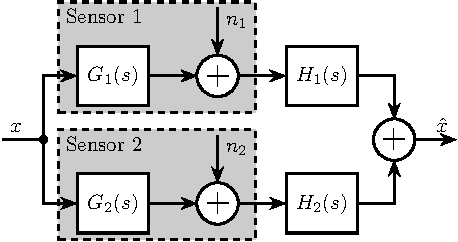
\includegraphics[scale=1]{figs/fusion_two_noisy_sensors_with_dyn_ter.pdf}
\caption{\label{fig:fusion_two_noisy_sensors_with_dyn_ter}
Sensor Fusion Architecture}
\end{figure}

We see that the complementary filters \(H_1(s)\) and \(H_2(s)\) operates only on the noise of the sensors.

Thus, this architecture permits to filter each of the sensors without introducing any distortion in the physical quantity to measure.

\begin{equation}
  \delta x = \hat{x} - x = H_1 n_1 + H_2 n_2
\end{equation}

Usually, the two sensors have higher noise levels over distinct yet complementary frequency regions. The two complementary filters are used to combine the filtered noise and yield to a better estimate \(\hat{x}\) over a larger bandwidth.

The noise of the super sensor is determine by the norm of the complementary filters.

\subsection{Noise Sensor Filtering}
\label{sec:orga5d7d56}
\label{sec:noise_filtering}

\subsection{Robustness of the Fusion}
\label{sec:org4ea42db}
\label{sec:fusion_robustness}

\subsection{Upper bounds as a mathematical translation of the requirements}
\label{sec:orgfad4c6f}
\label{sec:requirements_upper_bounds}

\textbf{The conclusion of the section should be that it is the norm of the complementary filter that is important and that is why we propose a method of synthesis based on H-infinity}

\section{Shaping of Complementary Filters using the \(\mathcal{H}_\infty\) Synthesis}
\label{sec:org25970ea}
\label{sec:hinf_method}
As shown in Sec. \ldots{}, most of the performance requirements can be expressed as upper bounds on the magnitude of the complementary filters.
As presented in Sec. \ref{sec:trans_perf}, almost all the requirements can be specified with upper bounds on the complementary filters.

Thus, the \(\mathcal{H}_\infty\) framework seems adapted and we here propose a technique to synthesis complementary filters while specifying uppers bounds on their magnitudes.

\subsection{\(\mathcal{H}_\infty\) problem formulation}
\label{sec:org7747d99}
\label{sec:hinf_synthesis}

In this section, we formulate the \(\hinf\) problem for the synthesis of complementary filters.

The synthesis objective is to shape an high pass filter \(H_H\) and a low pass filter \(H_L\) while ensuring their complementary property (\(H_H + H_L = 1\)).

To do so, we define two weighting functions \(w_L\) and \(w_H\) that will respectively used to shape \(H_L\) and \(H_H\).

The synthesis problem is then
\begin{subnumcases}{\text{Find } H_L, H_H \text{ such that}}
  H_L \text{ and } H_H \text{ are stable} \label{eq:hinf_cond_stability}\\
  H_L + H_H = 1 \label{eq:hinf_cond_complementarity} \\
  |w_L H_L| \le 1 \quad \forall\omega \label{eq:hinf_cond_hl} \\
  |w_H H_H| \le 1 \quad \forall\omega \label{eq:hinf_cond_hh}
\end{subnumcases}


To express this synthesis problem into an \(\hinf\) synthesis problem, we define the following generalized plant \(P\) (also shown on Fig. \ref{fig:sf_hinf_filters_plant_b}):
\begin{equation}
\label{eq:generalized_plant}
  \colvec{w\\u} = P \colvec{z_H \\ z_L \\ v}; \quad P = \begin{bmatrix} w_H & -w_H \\ 0 & w_L \\ 1 & 0 \end{bmatrix}
\end{equation}

\begin{figure}[htbp]
\centering
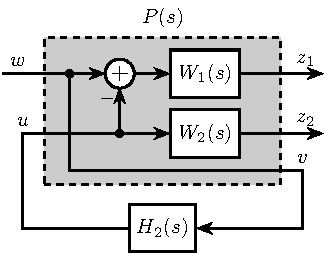
\includegraphics[scale=1]{figs/h_infinity_robust_fusion.pdf}
\caption{\label{fig:h_infinity_robust_fusion}
Architecture used for the \(\mathcal{H}_\infty\) synthesis of complementary filters}
\end{figure}

The \(\hinf\) synthesis objective is then to design a stable filter \(H_L\) (Fig. \ref{fig:sf_hinf_filters_b}) such that the \(\mathcal{H}_\infty\) norm of the transfer function from \(w\) to \([z_H, \ z_L]\) is less than \(1\):
\begin{equation}
  \hnorm{\begin{matrix} (1 - H_L) w_H \\ H_L w_L \end{matrix}} \le 1
\end{equation}
Which is equivalent to
\begin{equation}
\label{eq:hinf_problem}
  \hnorm{\begin{matrix} H_H w_H \\ H_L w_L \end{matrix}} < 1 \text{ by choosing } H_H = 1 - H_L
\end{equation}

Performance conditions \eqref{eq:hinf_cond_hl} and \eqref{eq:hinf_cond_hl} are satisfied by \eqref{eq:hinf_problem}.
Complementary condition \eqref{eq:hinf_cond_complementarity} is satisfied by design: \(H_H = 1 - H_L\) and thus \(H_L + H_H = 1\).
The stability condition \eqref{eq:hinf_cond_stability} is guaranteed by the \(H_\infty\) synthesis (\textbf{reference}).


Using this synthesis method, we are then able to shape at the same time the high pass and low pass filters while ensuring their complementary.

\subsection{Choice of the weighting functions}
\label{sec:org3997457}
\label{sec:hinf_weighting_func}

We here give some advice on the design of the weighting functions used for the synthesis of the complementary filters using the \(\mathcal{H}_\infty\) method.

The weighting functions should be such that the performance requirements are met as explain in Sec. \ref{sec:trans_perf}.

However, one should be careful when designing the complementary filters, and should only use stable and minimum phase transfer functions.
The order of the weights should stay reasonably small as this will increase the complexity of the optimization problem.

Moreover, the order of the complementary filters will be equal to the sum of the order of the weighting functions used.

One should not forget the fundamental limitations imposed by the synthesis: \(H_L(s) + H_H(s) = 1\).
This implies that \(H_L\) and \(H_H\) cannot be made small at the same time.


We here propose a formula for the design of the weighting function \eqref{eq:weight_formula}.

\begin{equation}
\label{eq:weight_formula}
  W(s) = \left(\frac{
           \hfill \frac{1}{\omega_0} \sqrt{\frac{1 - \left(\frac{G_0}{G_c}\right)^{\frac{2}{n}}}{1 - \left(\frac{G_c}{G_\infty}\right)^{\frac{2}{n}}}} s + \left(\frac{G_0}{G_c}\right)^{\frac{1}{n}}
         }{
           \left(\frac{1}{G_\infty}\right)^{\frac{1}{n}} \frac{1}{\omega_0} \sqrt{\frac{1 - \left(\frac{G_0}{G_c}\right)^{\frac{2}{n}}}{1 - \left(\frac{G_c}{G_\infty}\right)^{\frac{2}{n}}}} s + \left(\frac{1}{G_c}\right)^{\frac{1}{n}}
         }}\right)^n
\end{equation}
with:
\begin{itemize}
\item \(G_0\) is the absolute gain at low frequency
\item \(G_\infty\) is the absolute gain at high frequency
\item \(\omega_0\) and \(G_c\) define the absolute value of the filter at \(\omega = \omega_0\): \(|W(j\omega_0)| = G_c\)
\item \(n\) is the absolute slope of the filter, it is also equal to the order of the filter
\end{itemize}

The constrains are that \(G_0 < 1 < G_\infty\) and \(G_0 < G_c < G_\infty\) or that \(G_\infty < 1 < G_0\) and \(G_\infty < G_c < G_0\).

The shape of the weight generated using the formula is shown on figure \ref{fig:weight_formula}.

\begin{figure}[htbp]
\centering
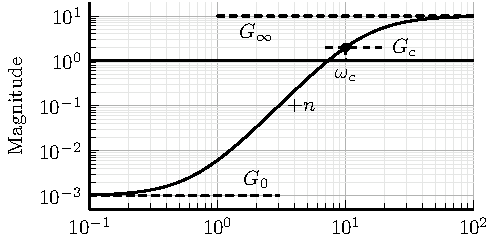
\includegraphics[scale=1]{figs/weight_formula.pdf}
\caption{\label{fig:weight_formula}
Amplitude of the proposed formula for the weighting functions, \(G_0 = 1e^{-3}\), \(G_\infty = 10\), \(\omega_c = \SI{10}{Hz}\), \(G_c = 2\), \(n = 3\)}
\end{figure}

\subsection{Example}
\label{sec:org27ef2a0}
\label{sec:hinf_example}

We are now using the proposed \(\mathcal{H}_\infty\) complementary filters synthesis method for a simple example.

The goal is to design

We use the formula \eqref{eq:weight_formula} for both \(w_L(s)\) and \(w_H(s)\).
The parameters used are summarized on table \ref{tab:weights_params}. And the magnitude of the weighting functions are shown on figure \ref{fig:weights_wl_wh}.

\begin{table}[!htpb]
\caption{\label{tab:weights_params}
Parameters used for the weighting functions}
\centering
\begin{tabular}{|l|X|X|}
\hline
Parameters & \(w_L\) & \(w_H\)\\
\hline
\(G_0\) & \(0.1\) & \(1000\)\\
\hline
\(G_\infty\) & \(1000\) & \(0.1\)\\
\hline
\(\omega_c\) [\(\si{Hz}\)] & \(11\) & \(10\)\\
\hline
\(G_c\) & \(2\) & \(2\)\\
\hline
\(n\) & \(2\) & \(3\)\\
\hline
\end{tabular}
\end{table}


\begin{figure}[htbp]
\centering
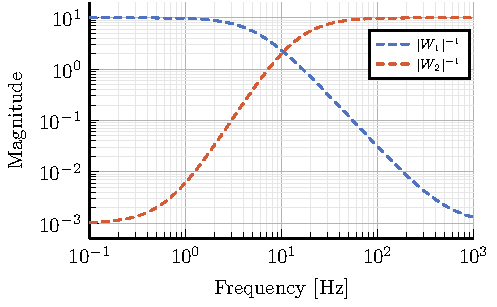
\includegraphics[scale=1]{figs/weights_wl_wh.pdf}
\caption{\label{fig:weights_wl_wh}
Weighting Functions used for the \(\mathcal{H}_\infty\) Synthesis}
\end{figure}

After synthesis, the obtain filters are:
\begin{align}
  H_L(s) &= \frac{10^{-8} (s+6.6e^9) (s+3450)^2 (s^2 + 49s + 895)}{(s+6.6e^4) (s^2 + 106 s + 3000) (s^2 + 72s + 3580)}\\
  H_H(s) &= \frac{(s+6.6e^4) (s+160) (s+4)^3}{(s+6.6e^4) (s^2 + 106 s + 3000) (s^2 + 72s + 3580)}
\end{align}

Their bode plot is shown on figure \ref{fig:hinf_synthesis_results}.

\begin{figure}[htbp]
\centering
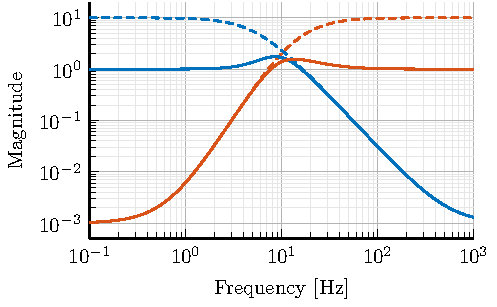
\includegraphics[scale=1]{figs/hinf_synthesis_results.pdf}
\caption{\label{fig:hinf_synthesis_results}
Obtain Complementary Filters}
\end{figure}

\subsection{Synthesis of Three Complementary Filters}
\label{sec:orgbc6a88d}
\label{sec:hinf_three_comp_filters}

We want:
\begin{align*}
  & |H_1 w_1| < 1, \quad \forall\omega\\
  & |H_2 w_2| < 1, \quad \forall\omega\\
  & |H_3 w_3| < 1, \quad \forall\omega\\
  & H_1 + H_2 + H_3 = 1
\end{align*}

The \(\mathcal{H}_\infty\) objective is:
\begin{align*}
  & |H_1 w_1| < 1, \quad \forall\omega\\
  & |H_2 w_2| < 1, \quad \forall\omega\\
  & |(1 - H_1 - H_2) w_3| < 1, \quad \forall\omega\\
\end{align*}

And thus if we choose \(H_3 = 1 - H_1 - H_2\) we have solved the problem.

\begin{figure}[htbp]
\centering
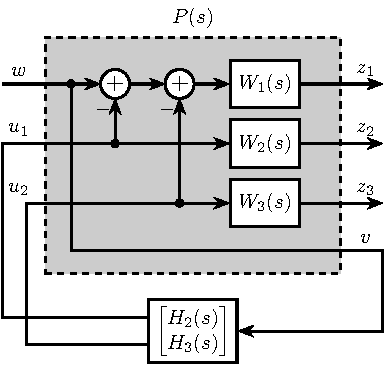
\includegraphics[scale=1]{figs/comp_filter_three_hinf.pdf}
\caption{\label{fig:comp_filter_three_hinf}
Architecture for the \(\mathcal{H}_\infty\) synthesis of three complementary filters}
\end{figure}

\begin{figure}[htbp]
\centering
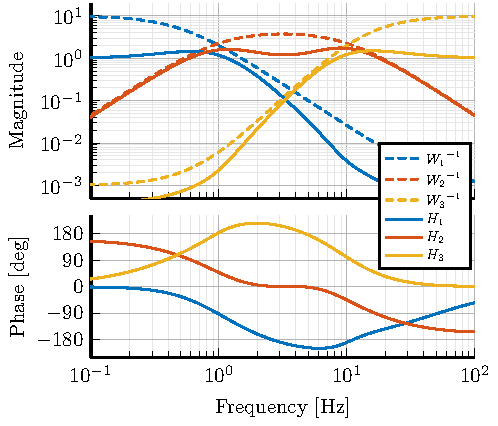
\includegraphics[scale=1]{figs/hinf_three_synthesis_results.pdf}
\caption{\label{fig:hinf_three_synthesis_results}
Obtained three complementary filters}
\end{figure}

\section{Application to the design of}
\label{sec:orgdde45d9}
\label{sec:application_ligo}

\subsection{Specifications}
\label{sec:org42c5fdc}
\label{sec:ligo_specifications}

\begin{figure}[htbp]
\centering
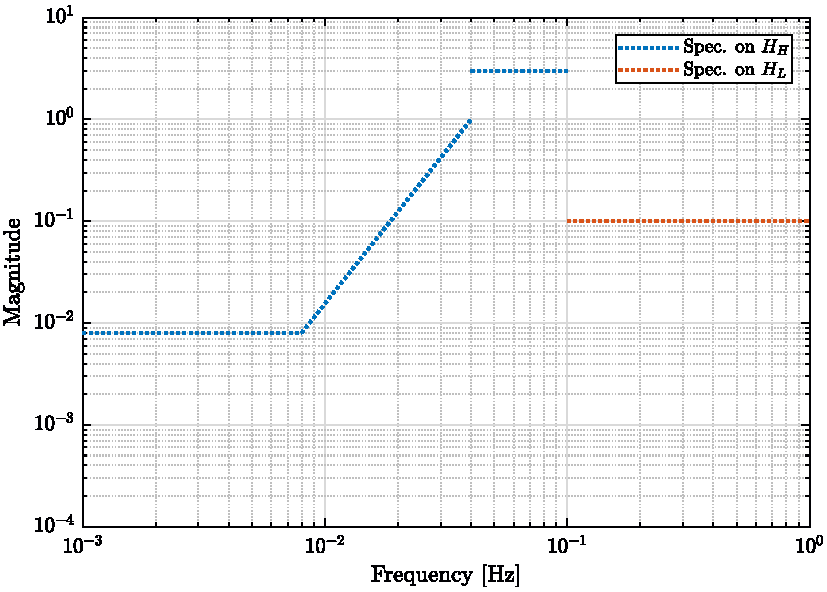
\includegraphics[scale=1]{figs/ligo_specifications.pdf}
\caption{\label{fig:ligo_specifications}
Specifications on the norms of the complementary filters}
\end{figure}

\subsection{Weighting functions design}
\label{sec:orgd835d49}
\label{sec:ligo_weights}

\begin{figure}[htbp]
\centering
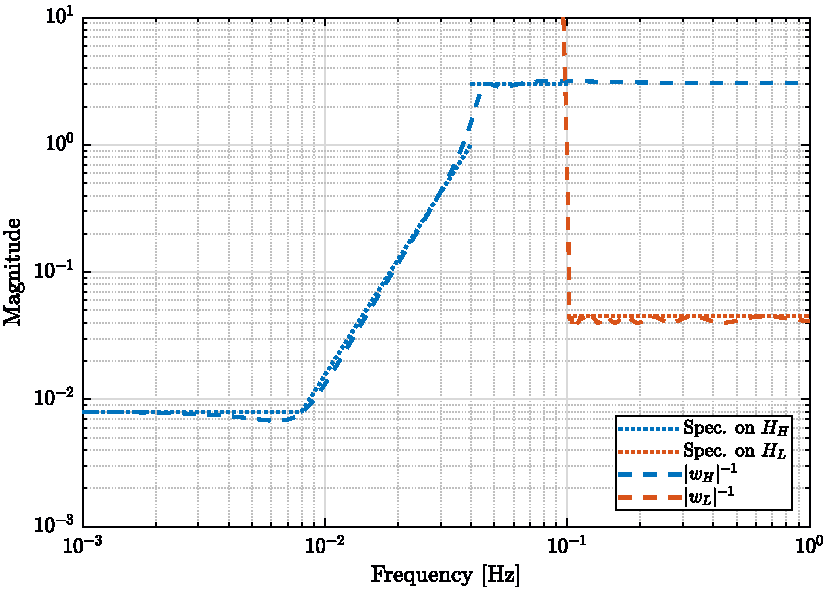
\includegraphics[scale=1]{figs/ligo_weights.pdf}
\caption{\label{fig:ligo_weights}
Weighting Functions used for the \(\mathcal{H}_\infty\) synthesis}
\end{figure}

\subsection{Comparison}
\label{sec:org7d0ba2b}
\label{sec:ligo_results}

\begin{figure}[htbp]
\centering
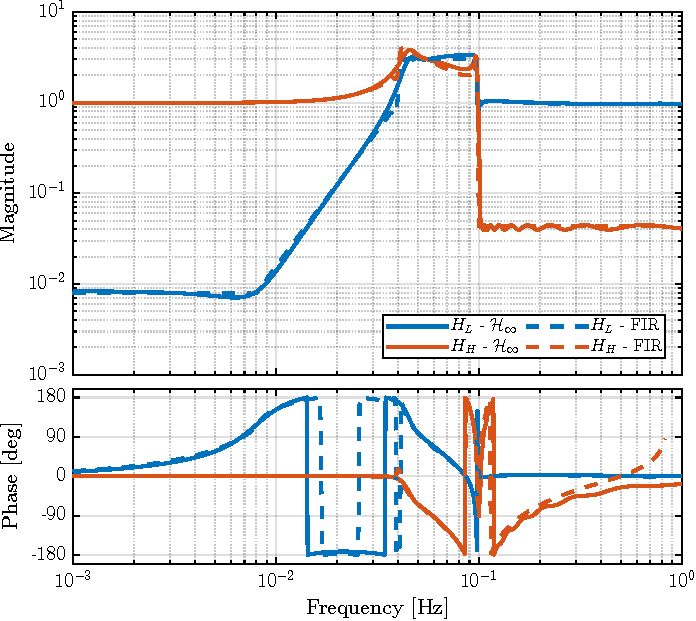
\includegraphics[scale=1]{figs/comp_fir_ligo_hinf.pdf}
\caption{\label{fig:comp_fir_ligo_hinf}
Comparison of the filters obtain with the \(\mathcal{H}_\infty\) synthesis and the FIR filters designed in \cite{hua05_low_ligo}}
\end{figure}

\section{Conclusion}
\label{sec:org64a0819}
\label{sec:conclusion}

\section{Acknowledgment}
\label{sec:orgc4f1f42}

\bibliography{ref}
\end{document}